\documentclass[
  shownotes,
  xcolor={svgnames},
  hyperref={colorlinks,citecolor=DarkBlue,linkcolor=andesred,urlcolor=DarkBlue}
  , aspectratio=169]{beamer}
\usepackage{animate}
\usepackage{amsmath}
\usepackage{amsfonts}
\usepackage{amssymb}
\usepackage{pifont}
\usepackage{mathpazo}
%\usepackage{xcolor}
\usepackage{multimedia}
\usepackage{fancybox}
\usepackage[para]{threeparttable}
\usepackage{multirow}
\setcounter{MaxMatrixCols}{30}
\usepackage{subcaption}
\usepackage{graphicx}
\usepackage{lscape}
\usepackage[compatibility=false,font=small]{caption}
\usepackage{booktabs}
\usepackage{ragged2e}
\usepackage{chronosys}
\usepackage{appendixnumberbeamer}
\usepackage{animate}
\setbeamertemplate{caption}[numbered]
\usepackage{color}
%\usepackage{times}
\usepackage{tikz}
\usetikzlibrary{arrows}
\usepackage{comment} %to comment
%% BibTeX settings
\usepackage{natbib}
\bibliographystyle{apalike}
\bibpunct{(}{)}{,}{a}{,}{,}
\setbeamertemplate{bibliography item}{[\theenumiv]}

% Defines columns for bespoke tables
\usepackage{array}
\newcolumntype{L}[1]{>{\raggedright\let\newline\\\arraybackslash\hspace{0pt}}m{#1}}
\newcolumntype{C}[1]{>{\centering\let\newline\\\arraybackslash\hspace{0pt}}m{#1}}
\newcolumntype{R}[1]{>{\raggedleft\let\newline\\\arraybackslash\hspace{0pt}}m{#1}}


\usepackage{xfrac}


\usepackage{multicol}
\setlength{\columnsep}{0.5cm}

% Theme and colors
\usetheme{Boadilla}

% I define a custom pallete
\definecolor{andesred}{HTML}{1B175E}
\definecolor{andesyellow}{HTML}{ffff00}

% Other options
\providecommand{\U}[1]{\protect\rule{.1in}{.1in}}
\usefonttheme{serif}
\setbeamertemplate{itemize items}[default]
\setbeamertemplate{enumerate items}[square]
\setbeamertemplate{section in toc}[circle]


\definecolor{mybackground}{HTML}{1B175E}
\definecolor{myforeground}{HTML}{0000A0}

\setbeamercolor{normal text}{fg=black,bg=white}
\setbeamercolor{alerted text}{fg=andesred}
\setbeamercolor{example text}{fg=black}

\setbeamercolor{background canvas}{fg=myforeground, bg=white}
\setbeamercolor{background}{fg=myforeground, bg=mybackground}
\setbeamercolor{palette tertiary}{fg=myforeground,bg=mybackground}

\setbeamercolor{palette primary}{fg=black, bg=white}
\setbeamercolor{palette secondary}{fg=black, bg=white!10!andesyellow}
\setbeamercolor{palette tertiary}{fg=black, bg=white}


\setbeamercolor{frametitle}{fg=black}
\setbeamercolor{title}{fg=black}
\setbeamercolor{block title}{fg=andesred}
\setbeamercolor{itemize item}{fg=andesred}
\setbeamercolor{itemize subitem}{fg=andesred}
\setbeamercolor{itemize subsubitem}{fg=andesred}
\setbeamercolor{enumerate item}{fg=andesred}
\setbeamercolor{item projected}{bg=gray!30!white,fg=andesred}
\setbeamercolor{enumerate subitem}{fg=andesred}
\setbeamercolor{section number projected}{bg=gray!30!white,fg=andesred}
\setbeamercolor{section in toc}{fg=andesred}
\setbeamercolor{caption name}{fg=andesred}
\setbeamercolor{button}{bg=gray!30!white,fg=andesred}
\setbeamercolor{title in head/foot}{fg=andesred}



\usepackage{fancyvrb}
\newcommand{\VerbBar}{|}
\newcommand{\VERB}{\Verb[commandchars=\\\{\}]}
\DefineVerbatimEnvironment{Highlighting}{Verbatim}{commandchars=\\\{\}}
% Add ',fontsize=\small' for more characters per line
\usepackage{framed}
\definecolor{shadecolor}{RGB}{248,248,248}
\newenvironment{Shaded}{\begin{snugshade}}{\end{snugshade}}
\newcommand{\AlertTok}[1]{\textcolor[rgb]{0.94,0.16,0.16}{#1}}
\newcommand{\AnnotationTok}[1]{\textcolor[rgb]{0.56,0.35,0.01}{\textbf{\textit{#1}}}}
\newcommand{\AttributeTok}[1]{\textcolor[rgb]{0.77,0.63,0.00}{#1}}
\newcommand{\BaseNTok}[1]{\textcolor[rgb]{0.00,0.00,0.81}{#1}}
\newcommand{\BuiltInTok}[1]{#1}
\newcommand{\CharTok}[1]{\textcolor[rgb]{0.31,0.60,0.02}{#1}}
\newcommand{\CommentTok}[1]{\textcolor[rgb]{0.56,0.35,0.01}{\textit{#1}}}
\newcommand{\CommentVarTok}[1]{\textcolor[rgb]{0.56,0.35,0.01}{\textbf{\textit{#1}}}}
\newcommand{\ConstantTok}[1]{\textcolor[rgb]{0.00,0.00,0.00}{#1}}
\newcommand{\ControlFlowTok}[1]{\textcolor[rgb]{0.13,0.29,0.53}{\textbf{#1}}}
\newcommand{\DataTypeTok}[1]{\textcolor[rgb]{0.13,0.29,0.53}{#1}}
\newcommand{\DecValTok}[1]{\textcolor[rgb]{0.00,0.00,0.81}{#1}}
\newcommand{\DocumentationTok}[1]{\textcolor[rgb]{0.56,0.35,0.01}{\textbf{\textit{#1}}}}
\newcommand{\ErrorTok}[1]{\textcolor[rgb]{0.64,0.00,0.00}{\textbf{#1}}}
\newcommand{\ExtensionTok}[1]{#1}
\newcommand{\FloatTok}[1]{\textcolor[rgb]{0.00,0.00,0.81}{#1}}
\newcommand{\FunctionTok}[1]{\textcolor[rgb]{0.00,0.00,0.00}{#1}}
\newcommand{\ImportTok}[1]{#1}
\newcommand{\InformationTok}[1]{\textcolor[rgb]{0.56,0.35,0.01}{\textbf{\textit{#1}}}}
\newcommand{\KeywordTok}[1]{\textcolor[rgb]{0.13,0.29,0.53}{\textbf{#1}}}
\newcommand{\NormalTok}[1]{#1}
\newcommand{\OperatorTok}[1]{\textcolor[rgb]{0.81,0.36,0.00}{\textbf{#1}}}
\newcommand{\OtherTok}[1]{\textcolor[rgb]{0.56,0.35,0.01}{#1}}
\newcommand{\PreprocessorTok}[1]{\textcolor[rgb]{0.56,0.35,0.01}{\textit{#1}}}
\newcommand{\RegionMarkerTok}[1]{#1}
\newcommand{\SpecialCharTok}[1]{\textcolor[rgb]{0.00,0.00,0.00}{#1}}
\newcommand{\SpecialStringTok}[1]{\textcolor[rgb]{0.31,0.60,0.02}{#1}}
\newcommand{\StringTok}[1]{\textcolor[rgb]{0.31,0.60,0.02}{#1}}
\newcommand{\VariableTok}[1]{\textcolor[rgb]{0.00,0.00,0.00}{#1}}
\newcommand{\VerbatimStringTok}[1]{\textcolor[rgb]{0.31,0.60,0.02}{#1}}
\newcommand{\WarningTok}[1]{\textcolor[rgb]{0.56,0.35,0.01}{\textbf{\textit{#1}}}}
\usepackage{graphicx}
\makeatletter

\makeatother




\AtBeginSection[]
{
    \begin{frame}
        \frametitle{Agenda}
        \tableofcontents[currentsection]
    \end{frame}
}



\AtBeginSubsection[]
{
    \begin{frame}
        \frametitle{Agenda}
        \tableofcontents[currentsubsection]
    \end{frame}
}




%%%%%%%%%%%%%%% BEGINS DOCUMENT %%%%%%%%%%%%%%%%%%


\begin{document}


\title{Árboles (CARTs), Bagging and Random Forests}
\subtitle{Big Data y Machine Learning para Economía Aplicada}
\date{}

\author[Sarmiento-Barbieri]{Ignacio Sarmiento-Barbieri}
\institute[Uniandes]{Universidad de los Andes}


\begin{frame}[noframenumbering]
\maketitle
\end{frame}


%----------------------------------------------------------------------% 


\begin{frame}
\frametitle{Motivación}


\begin{itemize}
    \item Queremos predecir:

    \begin{align}
    Price=f(structural\,attributes,amenities,...)
    \end{align}
    \medskip
    \begin{itemize}
      \item Podemos aplicar linear regression,
    \end{itemize}
    \begin{align}
    Price=\beta_0 + \beta_1 Habitaciones + \beta_2 DCBD + u
    \end{align}
  \medskip

  \item Aplicar OLS a este problema requiere tomar algunas decisiones.
  


\end{itemize}
\end{frame}
%----------------------------------------------------------------------% 
\begin{frame}
\frametitle{Motivación}

 \begin{figure}[H] \centering
            \captionsetup{justification=centering}
              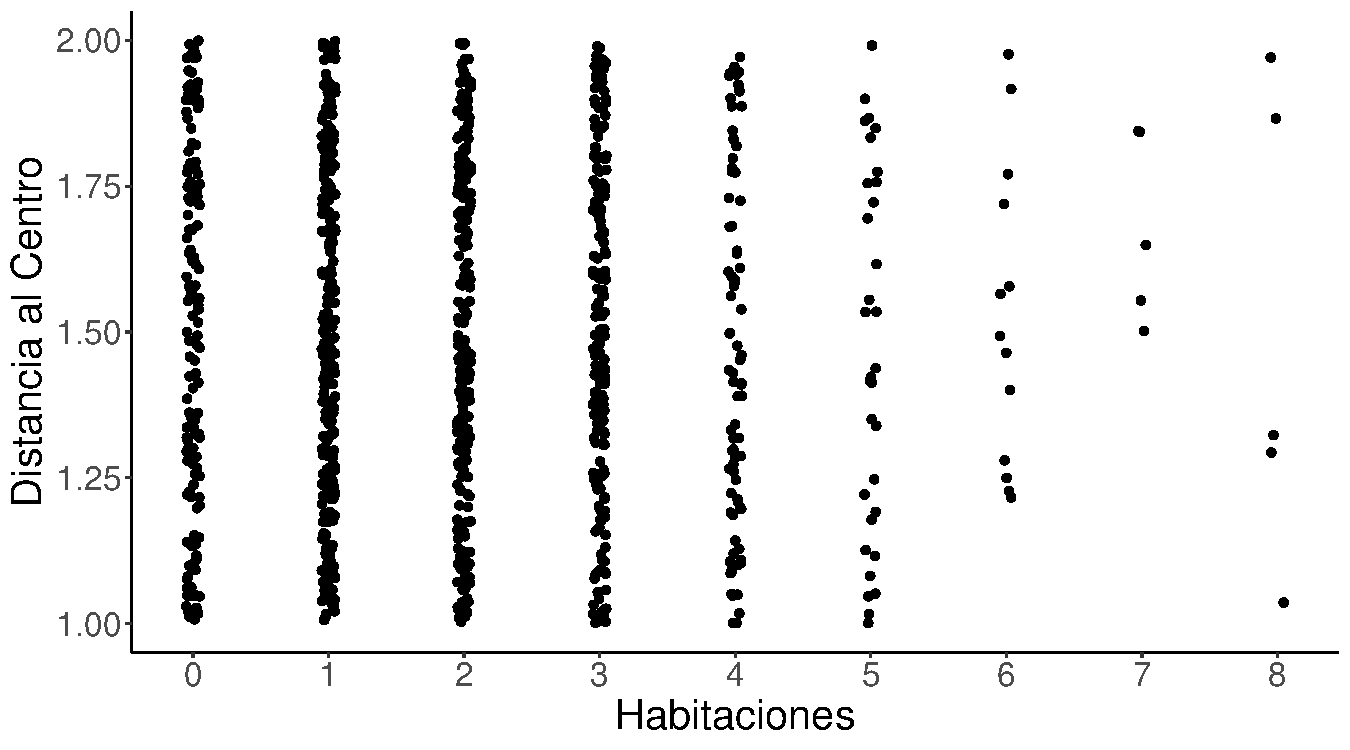
\includegraphics[scale=0.35]{figures/dcbd_hab.pdf}                           
 \end{figure}


\end{frame}
%----------------------------------------------------------------------%
%----------------------------------------------------------------------%
\section{Árboles}
%----------------------------------------------------------------------%
%----------------------------------------------------------------------%
\subsection{¿Qué hacen?}
%----------------------------------------------------------------------%
%----------------------------------------------------------------------%
\begin{frame}[fragile]
\frametitle{¿Qué hacen?}


\begin{columns}[T] % align columns
\begin{column}{.48\textwidth}
  
\begin{enumerate}
    \footnotesize
\item Y es la variable a predecir, los insumos son $X_1$ y $X_2$
\medskip
\item  Partimos el espacio $(X_1,X_2)$ en dos regiones, en base a una sola variable .
\medskip
\item Punto: elegir la variable y el punto de partición de manera óptima.
\end{enumerate}


\end{column}  
\hfill
\begin{column}{.52\textwidth}

 \begin{tikzpicture}
 \draw (3,3) rectangle (8,8);
 \node[rotate=90] at (2,6) {$DCBD$};
 \node at (2.7,5.5) {$s_1$};
  \node[] at (6,2) {$Habitaciones$};
    \draw[dashed] (3,5.5) -- (8,5.5);
  
\end{tikzpicture}
\end{column}
\end{columns}

\end{frame}


%----------------------------------------------------------------------%
\begin{frame}[fragile]
\frametitle{¿Qué hacen?}


\begin{columns}[T] % align columns
\begin{column}{.48\textwidth}
  
\begin{enumerate}
    \footnotesize
\item Y es la variable a predecir, los insumos son $X_1$ y $X_2$
\medskip
\item  Partimos el espacio $(X_1,X_2)$ en dos regiones, en base a una sola variable .
\medskip
\item Punto: elegir la variable y el punto de partición de manera óptima.
\medskip
\item Continuamos partiendo
\end{enumerate}


\end{column}  
\hfill
\begin{column}{.52\textwidth}

 \begin{tikzpicture}
 \draw (3,3) rectangle (8,8);
 \node[rotate=90] at (2,6) {$DCBD$};
 \node at (2.7,5.5) {$s_1$};
  \node[] at (6,2) {$Habitaciones$};
  \node at (5,2.7) {$s_2$};
  \draw[dashed] (3,5.5) -- (8,5.5);
  \draw[dashed] (5,5.5) -- (5,8);
\end{tikzpicture}
\end{column}
\end{columns}

\end{frame}
%----------------------------------------------------------------------%
\begin{frame}[fragile]
\frametitle{¿Qué hacen?}


\begin{columns}[T] % align columns
\begin{column}{.42\textwidth}
  
\begin{enumerate}
    \footnotesize
\item Y es la variable a predecir, los insumos son $X_1$ y $X_2$
\medskip
\item  Partimos el espacio $(X_1,X_2)$ en dos regiones, en base a una sola variable .
\medskip
\item Punto: elegir la variable y el punto de partición de manera optima (mejor ajuste global.
\medskip
\item Continuamos partiendo
\end{enumerate}


\end{column}  
\hfill
\begin{column}{.48\textwidth}

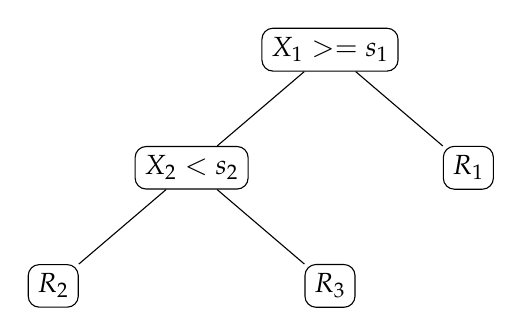
\begin{tikzpicture}[sibling distance=10em,
  every node/.style = {shape=rectangle, rounded corners,
    draw, align=center,
    top color=white, bottom color=white}]]
  \node {$X_1 >= s_1$}
   child { node {$X_2 < s_2$} 
            child{node {$R_2$}}
            child{node {$R_3$}}}
  child { node {$R_1$} };
   
    
\end{tikzpicture}

\end{column}
\end{columns}


\end{frame}

%----------------------------------------------------------------------%
\begin{frame}[fragile]
\frametitle{¿Qué hacen?}




  
\begin{columns}[T] % align columns
\begin{column}{.42\textwidth}
  
\begin{figure}[H] \centering
            \captionsetup{justification=centering}
              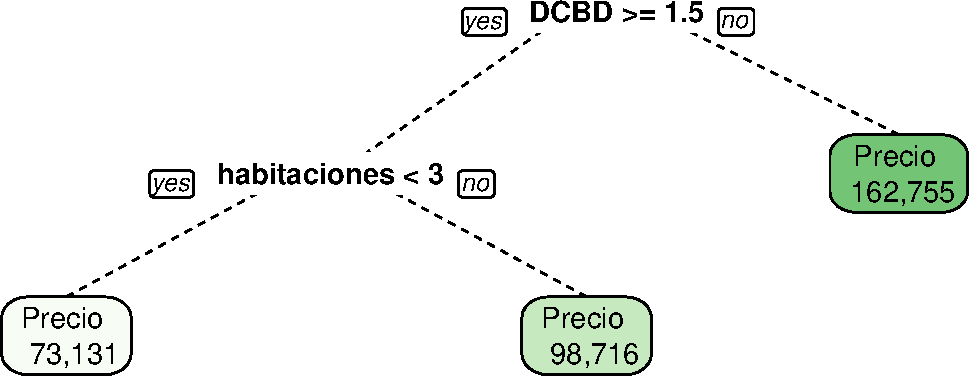
\includegraphics[scale=0.4]{figures/trees.pdf}                           
 \end{figure}

\end{column}  
\hfill
\begin{column}{.48\textwidth}

 \begin{figure}[H] \centering
            \captionsetup{justification=centering}
              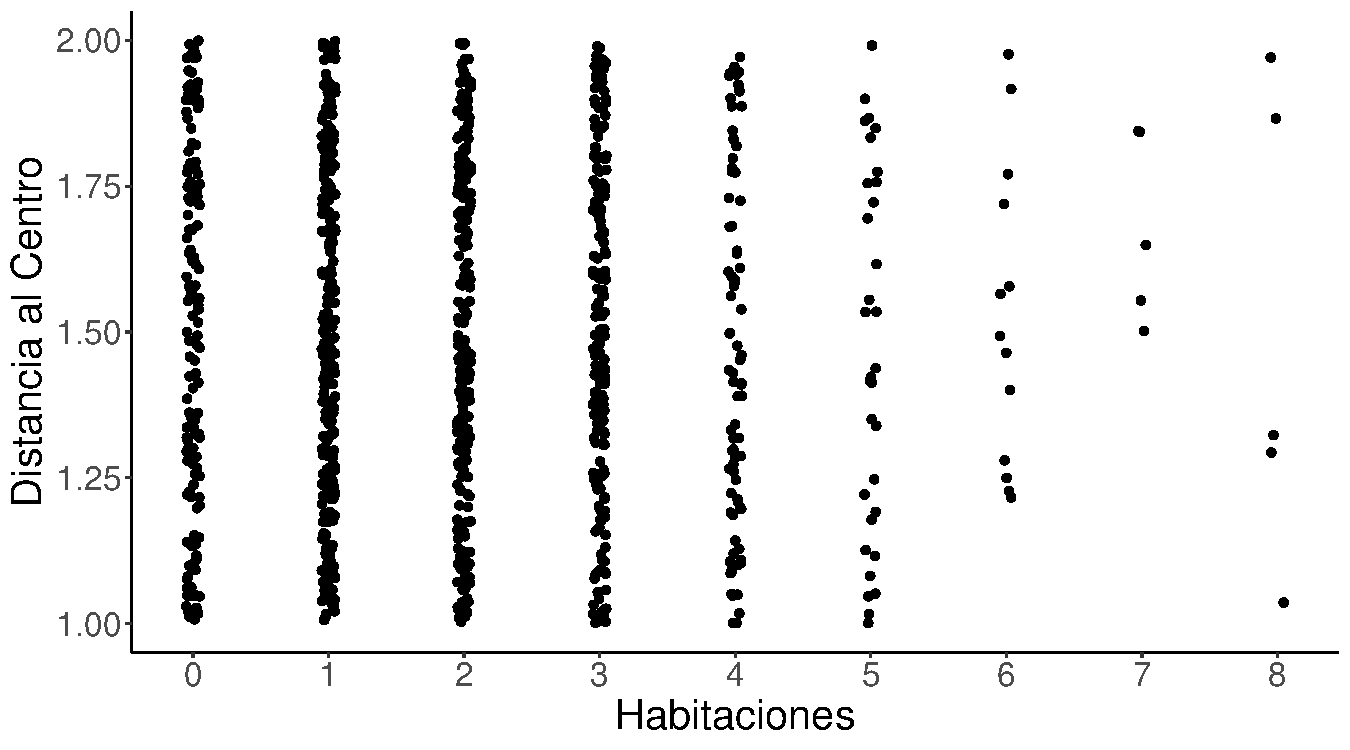
\includegraphics[scale=0.25]{figures/dcbd_hab.pdf}                           
 \end{figure}

\end{column}
\end{columns}

\end{frame}


%----------------------------------------------------------------------%
%----------------------------------------------------------------------%
\subsection{¿Cómo lo hacen?}
%----------------------------------------------------------------------%

%----------------------------------------------------------------------%
\begin{frame}[fragile]
\frametitle{¿Cómo construimos un árbol de decisión?}


\begin{itemize}
\item Datos: $y_{n\times 1}$  y $X_{n\times k}$ 
\medskip
\item Definiciones
\medskip
\begin{itemize}
\item $j$ es la variable que parte el espacio y  $s$ es el punto de partición
\medskip
\item Defina los siguientes semiplanos
\begin{align}
R_1(j,s)=\{X|X_j\leq s\} \,\,\, \& \,\,\, R_2(j,s)=\{X|X_j > s\}
\end{align}
\item El problema: buscar la variable de partición $X_j$ y el punto $s$ de forma tal que 
\begin{align}
\underset{j,s}{min} \left[ \underset{y_{R_1}}{min}\sum_{x_i\in R_1(j,s)}(y-y_{R_1})^2+ \underset{y_{R_2}}{min}\sum_{x_i\in R_2(j,s)}(y-y_{R_2})^2\right]
\end{align}
\end{itemize}
\end{itemize}
\end{frame}
%----------------------------------------------------------------------%
\begin{frame}[t]
\frametitle{¿Cómo construimos un árbol de decisión?}

  \begin{itemize}
\item ¿Cuál es la solución?

\end{itemize}
\end{frame}

%----------------------------------------------------------------------%
\begin{frame}[fragile]
\frametitle{¿Cómo construimos un árbol de decisión?}
\begin{figure}[H] \centering
  \centering
  
\includegraphics[scale=0.35]{figures/baticomputer_meme.jpg}
  \\
  \tiny photo from \url{https://www.dailydot.com/parsec/batman-1966-labels-tumblr-twitter-vine/}
\end{figure}


\end{frame}
%----------------------------------------------------------------------%
\subsection{Sobreajuste}
%----------------------------------------------------------------------%
\begin{frame}[fragile]
\frametitle{Sobreajuste}


  
\begin{figure}[H] \centering
            \captionsetup{justification=centering}
              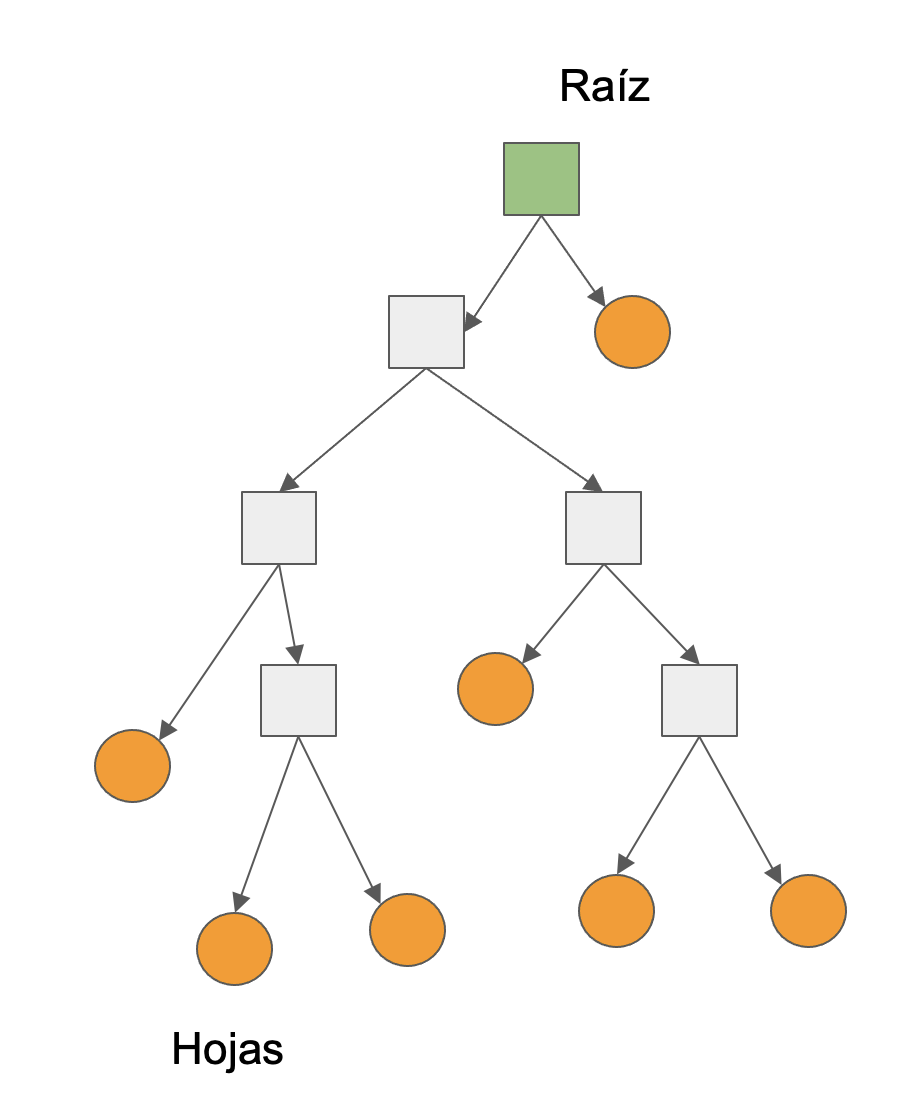
\includegraphics[scale=0.4]{figures/tree_uba.png}
 \end{figure}

\end{frame}
%----------------------------------------------------------------------%
\begin{frame}[fragile]
\frametitle{Sobreajuste. Algunas soluciones}

\begin{itemize}
  \item Fijar la profundidad del árbol.
  \medskip
  \item Fijar la cantidad de hojas (nodos terminales, regiones).
  \medskip
  \item Fijar la mínima cantidad de datos que están contenidos dentro de cada hoja. 
\medskip
\item  Pruning (poda).
\medskip
  \begin{itemize}
     \item Dejar crecer un árbol muy grande $T_0$
     \medskip
     \item Luego cortarlo obteniendo sub-árbol ({\it subtree})
     \medskip
     \item Como cortarlo? 
  \end{itemize}
\end{itemize}


\end{frame}
%----------------------------------------------------------------------%
\begin{frame}[fragile]
\frametitle{Pruning (poda)}

\begin{itemize}
\item No es posible calcular el error de predicción usando cross-validation para cada sub-árbol posible 
\medskip
\item Solución: {\it Cost complexity pruning (cortar las ramas mas débiles)}
\medskip
\begin{itemize}
    \item Indexamos los arboles con  $T$.
    \medskip
    \item Un sub-árbol $T \in T_0$ es un árbol que se obtuvo colapsando los nodos terminales de otro árbol (cortando ramas).
    \medskip
    \item  $[T]$ = número de nodos terminales del árbol  $T$
\end{itemize}
\end{itemize}
\end{frame}
%----------------------------------------------------------------------%
\begin{frame}[fragile]
\frametitle{Pruning (poda)}

\begin{itemize}
\item Cost complexity del árbol  $T$
\begin{align}
  C_{\alpha}(T)= \sum_{m=1}^{[T]} n_m Q_m (T) + \alpha [T]
\end{align}

  \begin{itemize}
  \item donde $Q_m (T)=\frac{1}{n_m} \sum_{x_i\in R_m} (y_i-\hat{y}_m)^2$ para los árboles de regresión
  \medskip
  \item  $Q_m (T)$ penaliza la heterogeneidad dentro de la regresión y el número de regiones 
  \medskip
  \item  Objetivo: para un dado $\alpha$, encontrar el pruning óptimo que minimice  $C_{\alpha}(T)$
  \end{itemize}
\end{itemize}
\end{frame}

%----------------------------------------------------------------------%
\begin{frame}[fragile]
\frametitle{Pruning (poda)}

\begin{itemize}
  \item Mecanismo de búsqueda para $T_\alpha$ ( pruning óptimo dado  $\alpha$).

\medskip
    \begin{quote}
    \centering
    Resultado: para cada  $\alpha$ hay un sub-árbol único  $T_\alpha$ que minimiza  C$\alpha$ (T).
    \end{quote}

\begin{itemize}

\medskip
\item Eliminar sucesivamente las ramas que producen un aumento mínimo en  $\sum_{m=1}^{[T]} n_m  Q_m (T)$
\medskip
\item Se colapsa hasta el nodo inicial pero va a través de una sucesión de árboles
\medskip
\item $T_\alpha$ pertenece a esta secuencia.  (Breiman et al., 1984)
\end{itemize}





\end{itemize}


\end{frame}
%----------------------------------------------------------------------%
\begin{frame}[fragile]
\frametitle{Pruning (poda)}
\framesubtitle{Algoritmo Completo}


\begin{enumerate}
  \item Utilizamos particiones recursivas binarias para hacer crecer el árbol
  \medskip
  \item Para un dado $\alpha$, aplicamos {\it cost complexity pruning} al árbol para obtener la secuencia de los subarboles como  $\alpha$.
  \medskip
  \item  Utilizamos K-fold cross-validation para elegir $\alpha$. 
  \medskip
  
  
\item Tenemos entonces una secuencia de subarboles para distintos valores de $\alpha$ 
\medskip
\item Elegimos el $\alpha$ y el subárbol que tienen el menor error de predicción.
\end{enumerate}


\end{frame}

%----------------------------------------------------------------------%
\begin{frame}[fragile]
\frametitle{Ejemplo}
\begin{figure}[H] \centering
  \centering
  
\includegraphics[scale=0.35]{figures/baticomputer_meme.jpg}
  \\
  \tiny photo from \url{https://www.dailydot.com/parsec/batman-1966-labels-tumblr-twitter-vine/}
\end{figure}

\end{frame}



%----------------------------------------------------------------------%
%----------------------------------------------------------------------%
\end{document}
%----------------------------------------------------------------------%
%----------------------------------------------------------------------%
